\documentclass{article}
\usepackage[utf8]{inputenc}
\usepackage{geometry}
\geometry{left=3cm,right=3cm,top=2cm,bottom=2cm}
\usepackage[utf8]{inputenc}
\usepackage{amsmath, amsfonts, amssymb, amsthm}
\usepackage[framemethod=TikZ]{mdframed}
\usepackage{mathrsfs}
\usepackage{comment}
\usepackage{enumerate}
\usepackage{xcolor}
\usepackage{titlesec}
\usepackage{setspace}
\usepackage[hidelinks,backref]{hyperref}
\usepackage{cleveref}
\usepackage[most]{tcolorbox}
\usepackage{ragged2e}
\usepackage{todonotes}
\usepackage{cleveref}
\usepackage{mathtools}

%
\titleformat*{\section}{\LARGE \bfseries}
\titleformat*{\subsection}{\Large \bfseries}
\titleformat*{\subsubsection}{\Large \bfseries}
% \titleformat*{\paragraph}{\large \bfseries}
\titleformat*{\subparagraph}{\large \bfseries}



% General 
\newcommand{\nextline}{\hfill\break}
\newcommand{\nl}{\nextline\rm}
% \newcommand{\placeholder}{{\bf\color{red} NOOOOOOT COMPLEEEEEEET! COOOOOOOM BAAAAAACK!!!}}
\newcommand{\placeholder}{\todo{NOOOOOOT COMPLEEEEEEET! COOOOOOOM BAAAAAACK!!!}}

\newcommand{\defeq}{\stackrel{def.}{=}}
% FA and LA
% inner product: \inne{a}{b}
\newcommand{\inne}[2]{\left<{#1},{#2}\right>}

% norm: \norm{a}
\newcommand{\norm}[1]{\left\|{#1}\right\|}

% Curly H
\newcommand{\hbs}{$\mathscr{H}$ }
\newcommand{\hbp}{\mathscr{H}}

% Dual : \dual{x}
\newcommand{\dual}[1]{{#1}^*}

% Sequence from 1  to infty: \sequ{x_n}
\newcommand{\sequ}[1]{\left({#1}\right)_1^\infty}

% f: A-> B \func{f}{A}{B}
\newcommand{\func}[3]{${#1}:{#2}\xrightarrow{}{#3}$}

% interior
\newcommand{\interior}{\textrm{int}}

% Bounded linear funcs
\newcommand{\blf}[2]{\mathcal{L}({#1},{#2})}

\newcommand{\prf}{\textit{proof}:   }



% Fields 
\newcommand{\real}{\mathbb{R}}
\newcommand{\comp}{\mathbb{C}}
\newcommand{\inte}{\mathbb{Z}}
\newcommand{\natu}{\mathbb{N}}





% Theorems
% \newtheorem{example}{Example}[subsection]
% \newtheorem{definition}[example]{Definition}
% \newtheorem{proposition}[example]{Proposition}
% \newtheorem{remark}[example]{Remark}
% \newtheorem{theorem}[example]{Theorem}
% \newtheorem{lemma}[example]{Lemma}
% \newtheorem{corollary}[example]{Corollary}


% for numbering the theorems            
\theoremstyle{plain}
%%%%%%%%%%%%%%%%%%%%%%%%%%%%%%%%%%%%%%%%%%%%%%%%%%%%%%%%%%%
\newtheorem{theorem}{Theorem}[section]
\newtheorem{lemma}[theorem]{Lemma}
\newtheorem{corollary}[theorem]{Corollary}
\newtheorem{proposition}[theorem]{Proposition}
%%%%%%%%%%%%%%%%%%%%%%%%%%%%%%%%%%%%%%%%%%%%%%%%%%%%%%%%%%%
% the following are not in italics
\theoremstyle{definition}
\newtheorem{definition}[theorem]{Definition}
\newtheorem{example}[theorem]{Example}
\newtheorem{remark}[theorem]{Remark}
\newtheorem{claim}[theorem]{Claim}
%%%%%%%%%%%%%%%%%%%%%%%%%%%%%%%%%%%%%%%%%%%%%%%%%%%%%%%%%%%%

% proof box
\newtcbtheorem[no counter]{pf}{Proof}{
  enhanced,
  rounded corners,
  attach boxed title to top,
  colback=white,
  colframe=black!25,
  fonttitle=\bfseries,
  coltitle=black,
  boxed title style={
    rounded corners,
    size=small,
    colback=black!25,
    colframe=black!25,
  } 
}{prf}

% extra content box to put in contents not covered in the lecture notes
% use the command \begin{unexaminable}
\newmdenv[skipabove=7pt, skipbelow=7pt,
    rightline=false, leftline=false, topline=false, bottomline=false,
    backgroundcolor = gray!10,
    innerleftmargin=1in, innerrightmargin=1in, innertopmargin=5pt,
    leftmargin=-1in, rightmargin=-1in, linewidth=4pt,
    innerbottommargin=5pt]{unexamBox}
\newenvironment{unexaminable}{\begin{unexamBox}}{\end{unexamBox}}


% clever ref settings
\crefname{lemma}{lemma}{lemmas}
\Crefname{lemma}{Lemma}{Lemmas}
\crefname{theorem}{theorem}{theorems}
\Crefname{theorem}{Theorem}{Theorems}

% formatting 
% https://tex.stackexchange.com/questions/217497/aligning-stackrel-signs-beneath-each-other-using-split
\newlength{\leftstackrelawd}
\newlength{\leftstackrelbwd}
\def\leftstackrel#1#2{\settowidth{\leftstackrelawd}%
{${{}^{#1}}$}\settowidth{\leftstackrelbwd}{$#2$}%
\addtolength{\leftstackrelawd}{-\leftstackrelbwd}%
\leavevmode\ifthenelse{\lengthtest{\leftstackrelawd>0pt}}%
{\kern-.5\leftstackrelawd}{}\mathrel{\mathop{#2}\limits^{#1}}}

\doublespacing
\RaggedRight
% modify innerrightmargin if floats were lost

\usepackage{amsfonts, amsmath, amssymb, amsthm, thmtools, bm}
\usepackage{avant} % Use the Avantgarde font for headings

% Boxed/framed environments
\newtheoremstyle{royalnumbox}%
{0pt}% Space above
{0pt}% Space below
{\normalfont}% Body font
{}% Indent amount
{\small\bf\sffamily\color{royal}}% Theorem head font
{\;}% Punctuation after theorem head
{0.25em}% Space after theorem head
{\sffamily \color{royal} 
    \thmname{#1} 
    \thmnumber{#2} \thmnote{\bfseries\color{black}---\nobreakspace#3.}} % Optional theorem note
\renewcommand{\qedsymbol}{$\blacksquare$}% Optional qed square

\newtheoremstyle{blacknumex}% Theorem style name
{5pt}% Space above
{5pt}% Space below
{\normalfont}% Body font
{} % Indent amount
{\small\bf\sffamily}% Theorem head font
{\;}% Punctuation after theorem head
{0.25em}% Space after theorem head
{\sffamily
    \thmname{#1}
    \thmnumber{#2}
    \thmnote{---\nobreakspace#3.}}% Optional theorem note

\newtheorem*{notation}{Notation}
\newtheorem*{hint}{Hint}
\newtheorem*{solution}{Solution}

\newcounter{dummy} 
\numberwithin{dummy}{section}

\theoremstyle{royalnumbox}
\newtheorem{definitionT}[dummy]{Definition}
\newtheorem{theoremT}[dummy]{Theorem}
\newtheorem{lemmaT}[dummy]{Lemma}
\newtheorem{corollaryT}[dummy]{Corollary}
\newtheorem{propositionT}[dummy]{Proposition}
\newtheorem{propertyT}[dummy]{Property}
\newtheorem{remarkT}[dummy]{Remark}

\theoremstyle{blacknumex}
\newtheorem{exampleT}[dummy]{Example}
\newtheorem{exerciseT}[dummy]{Exercise}

\numberwithin{equation}{section}

\RequirePackage[framemethod=default]{mdframed}

% Definition box
\newmdenv[skipabove=7pt, skipbelow=7pt,
rightline=false, leftline=true, topline=false, bottomline=false,
backgroundcolor = reddish!10, 
linecolor=reddish,
innerleftmargin=5pt, innerrightmargin=30pt, innertopmargin=5pt,
leftmargin=0cm, rightmargin=0cm, linewidth=4pt,
innerbottommargin=5pt]{dBox}

% Main Theorem box
\newmdenv[skipabove=7pt, skipbelow=7pt,
rightline=false, leftline=true, topline=false, bottomline=false,
backgroundcolor=c0!10, 
linecolor=c0,
innerleftmargin=5pt, innerrightmargin=30pt, innertopmargin=5pt,
leftmargin=0cm, rightmargin=0cm, linewidth=4pt, innerbottommargin=5pt]{tBox}

% Lemma/Corollary/Proposition/Property box
\newmdenv[skipabove=7pt, skipbelow=7pt,
rightline=false, leftline=true, topline=false, bottomline=false,
backgroundcolor = c0!10, 
linecolor=c0!80,
innerleftmargin=5pt, innerrightmargin=30pt, innertopmargin=5pt,
leftmargin=0cm, rightmargin=0cm, linewidth=4pt,
innerbottommargin=5pt]{lBox}

% Example/Remark/Exercise box
\newmdenv[skipabove=7pt, skipbelow=7pt,
rightline=false, leftline=true, topline=false, bottomline=false,
backgroundcolor = mossgreen!10!white,
linecolor = mossgreen,
innerleftmargin=5pt, innerrightmargin=30pt, innertopmargin=5pt,
leftmargin=0cm, rightmargin=0cm, linewidth=4pt,
innerbottommargin=5pt]{exBox}

% Proof box
% \newmdenv[skipabove=7pt, skipbelow=7pt,
% rightline=false, leftline=true, topline=false, bottomline=false,
% linecolor=gray,
% innerleftmargin=5pt, innerrightmargin=30pt, innertopmargin=5pt,
% leftmargin=0cm, rightmargin=0cm, linewidth=4pt,
% innerbottommargin=5pt]{proofBox}



% Creates an environment for each type of theorem and assigns it a theorem text style from the "Theorem Styles" section above and a colored box from above
\newenvironment{definition}{\begin{dBox}\begin{definitionT}}{\end{definitionT}\end{dBox}}
\newenvironment{theorem}{\begin{tBox}\begin{theoremT}}{\end{theoremT}\end{tBox}}
\newenvironment{lemma}{\begin{lBox}\begin{lemmaT}}{\end{lemmaT}\end{lBox}}
\newenvironment{proposition}{\begin{lBox}\begin{propositionT}}{\end{propositionT}\end{lBox}}
\newenvironment{corollary}{\begin{lBox}\begin{corollaryT}}{\end{corollaryT}\end{lBox}}
\newenvironment{property}{\begin{lBox}\begin{propertyT}}{\end{propertyT}\end{lBox}}


% \newenvironment{proof*}{\begin{proofBox}\begin{proof}}{\end{proof}\end{proofBox}}
\newenvironment{exercise}{\begin{exBox}\begin{exerciseT}}{\hfill{\color{royal}}\end{exerciseT}\end{exBox}}
\newenvironment{remark}{\begin{exBox}\begin{remarkT}}{\end{remarkT}\end{exBox}}
\newenvironment{example}{\begin{exBox}\begin{exampleT}}{{}\end{exampleT}\end{exBox}}
\title{Week 8}

\begin{document}  
\author{\aut}
\maketitle
\section{Weak vs. Strong topologies}
Let $(X, || \cdot ||_X)$ be a normed linear space with dual space $X^*$ (over $\mathbb{R}$).

\begin{definition}[Weak Convergence]\nl
A sequence $(x_n) \subset X$ \textbf{converges weakly} to $x\in X$, written as $x_n \xrightarrow{\text{w}} x (n \rightarrow \infty)$, if $\forall l \in X^*$, 
    $$\lim_{n\rightarrow \infty} \ell(x_n) = \ell(x);$$
$(x_n)$ \textbf{converges (strongly/in norm)} to $x$ if $\lim_{n\rightarrow \infty} ||x_n - x|| = 0$, write as: $x_n \rightarrow x (n\rightarrow \infty).$
\end{definition}

\begin{remark}
\label{properties of weak convergence}
We have the following remarks about weak convergence.  

\begin{enumerate}[1)]
    \item $x_n\rightarrow x$ implies  $x_n \xrightarrow{w} x$: $|\ell(x_n) - \ell(x)| \leq ||\ell||_* ||x_n - x||$
    
    \item The converse of 1) is false. Let $x_n (= e_n) = (0,...,0,1,0,...) \in l^2$. $||x_n-x_m|| = \sqrt{2}, n\neq m$, so $x_n$ doesn't converge (strongly). But $x_n \xrightarrow{w} 0$: by Riesz Representation, $\ell(\cdot) = \inne{y}{\cdot}_{l^2}$ for some $y \in l^2$, Hence with $y=(y^n)_n$, $$\ell(x_n) = \inne{y}{x_n} = y^n \leq \sqrt{\Sigma_{k\geq n} {|y^k|}^2} \xrightarrow{n\rightarrow \infty} 0$$, since $||y||_2 < \infty$.
    
    \item If $x_n \xrightarrow{w} x, x_n \xrightarrow{w} y$, then $x=y$. Assume not, \cref{dual elements separate points}, $\exists l \in X^*: \ell(x) \neq \ell(y)$ if $x\neq y$. With this $l$: $$\ell(x) = \lim_{n \to \infty} \ell(x_n) = \ell(y) $$ 
    ,a contradiction.
    
    \item $x_n \xrightarrow{w} x \Rightarrow \sup||x_n|| < \infty$. Consider $A_n \in \mathfrak{L}(X^*, \mathbb{R})$ ($=X^{**}$, the bidual) with $A_n(\ell) := \ell(x_n), \ell \in X^*$. $x_n \xrightarrow{w} x$ implies $\sup_n |A_n(l)| < \infty,$ $\forall l\in X^*$, and $X^*$ is complete so by Banach-Steinhaus: $$\sup_n ||A_n||_{\mathfrak{L}(X^*, \mathbb{R})} < \infty$$ 
    
    But by \Cref{dual characterisation of norm},  $||A_n||_{\mathfrak{L}(X^*,\mathbb{R})} = \sup_{l\in X^*, ||\ell||\leq 1} |\ell(x_n)| = ||x_n||_X$.
\end{enumerate}
\end{remark}

This naturally leads to:

\begin{definition}[Bidual]
\label{bidual defnition}
    $X^{**} := (X^*)^* \quad (=\mathfrak{L}(X^*,\mathbb{R}))$ is called \textbf{bidual} of $X$. $X$ embeds canonically into $X^{**}$ via: $$ \iota : X\rightarrow X^{**}: \iota(x)(\ell) := \ell(x) \quad \forall x \in X, \ell \in X^*$$ 
\end{definition}
\begin{remark}
    $\iota$ is a linear isometry: similarly as in \Cref{properties of weak convergence} 4) above. One has: $$\forall x \in X: ||x||_X = \sup_{l\in X^*, ||\ell|| \leq 1} |\ell(x)| = ||\iota(x)||_{**}$$
\end{remark}

\begin{definition}[Reflexive]\nl
    The space $X$ is reflexive if $\iota$ in \Cref{bidual defnition} is surjective.
\end{definition}

\begin{example}
\label{reflexive examples}
Some examples of reflexive spaces.  
\begin{enumerate}
    \item if $\dim X<\infty$, $X$ is reflexive;
    \item $H$ a Hilbert space is reflexive;
    \item $L^p, 1<p<\infty$ is reflexive;
    \item $L^1, L^\infty$ are in general not reflexive.
\end{enumerate}
\end{example}

\begin{proposition}
\label{non-reflexive space}
    $L^1[-1,1]$ and $L^{\infty}[-1,1]$ are not reflexive.
\end{proposition}
\begin{proof}
Consider $L^\infty[-1,1]$. 

Define the Dirac function 
$$\delta_{x_0}: C^0[-1,1] \rightarrow \mathbb{R}: f \mapsto \delta_{x_0}(f) = f(x_0)$$

$\delta_{x_0}$ is linear and continuous on $(C^0[-1,1],||\cdot ||_\infty)$. By \Cref{same norm extension}, there exists extension 
$$\ell\in (L^\infty [-1,1])^* \qquad \text{and} \qquad \ell\mid_{C^0[0,1]} = \delta_{x_0}.$$
with the same norm (Omit \textquotedblleft $[-1,1]$" henceforth) \\

For $g\in L^1$, we define $\forall f\in L^\infty$

$$\ell_g(f) = \int_{-1}^1 gf dx$$
then $l_g\in (L^\infty)^*$.

% \begin{unexaminable}
% This is the canonical embedding of $L^1$ into $(L^1)^{**}=(L^{\infty})^*$, since $(L^1)^* = L^{\infty}$, every $\zeta \in (L^1)^*$ can be written as  
% $$
% \zeta(g) = \int fg d\mu
% $$
% for some $f \in L^{\infty}$.  
% So $\iota: L^1 \mapsto (L^{\infty})^*:  \iota(g)(\zeta)=\zeta(g)$
% \end{unexaminable}

\textbf{Claim:} $\nexists g\in L^1: \ell=\ell_g$.  

The claim implies that $\iota: L^1 \rightarrow (L^1)^{**}=(L^\infty)^*, g \mapsto \ell_g$ is not surjective, i.e., $L^1$ is not reflexive.  

For $L^\infty$, use: $X$ reflexive $\Rightarrow$ $X^*$ reflexive (exercise).  

\textbf{Proof of Claim:} Suppose $\exists g\in L^1$ s.t. $l=l_g$. For simplicity let $x_0=0$.\\
Pick a bump function $\phi \in C^\infty [-1,1]: 0 \leq \phi \leq 1$

$$
\phi(x) = 1, \ x \in [-\frac{1}{2}, \frac{1}{2}] \qquad \text{and} \qquad \phi(x)=0, \ x=\pm 1
$$

For $n\leq 1: \phi_n(x) := \phi(nx)$. Then $0\leq \phi_n \leq 1$, $\phi_n \rightarrow 0 \ a.e.$.\\
This yields: $$1 = \phi_n(0)=\delta_{0}(\phi_n) = \ell(\phi_n) = l_g(\phi_n) = \int_{-1}^1 g\phi_n dx \rightarrow 0$$
this is a contradiction.
\end{proof}
\begin{unexaminable}
%     An example of a bump function is given at \href{https://math.stackexchange.com/questions/101480/are-there-other-kinds-of-bump-functions-than-e-frac1x2-1}{\color{navyblue} here}.  \\
% \begin{figure}[H]
%   \centering
%   \makebox[0pt]{%
%   \includesvg[inkscapelatex=false, width=0.5\paperwidth]{Chapter/Figures/bump_function.svg}
%   }
%   \caption{A bump function}
% \end{figure} 
An example of a bump function is given below:
\begin{equation}
f_n(x)=
\left\{
\begin{aligned}
&0 &|x|<\frac{1}{2n}\\
&{\rm exp}(1-\frac{1}{1-(2n|x|-1)^2}) &\frac{1}{2n}<|x|<\frac{1}{n}\\
&1 &\frac{1}{n}<|x|\leq1\\
\end{aligned}
\right.
\end{equation}


\begin{figure}[H]
  \centering
  \makebox[0pt]{%
  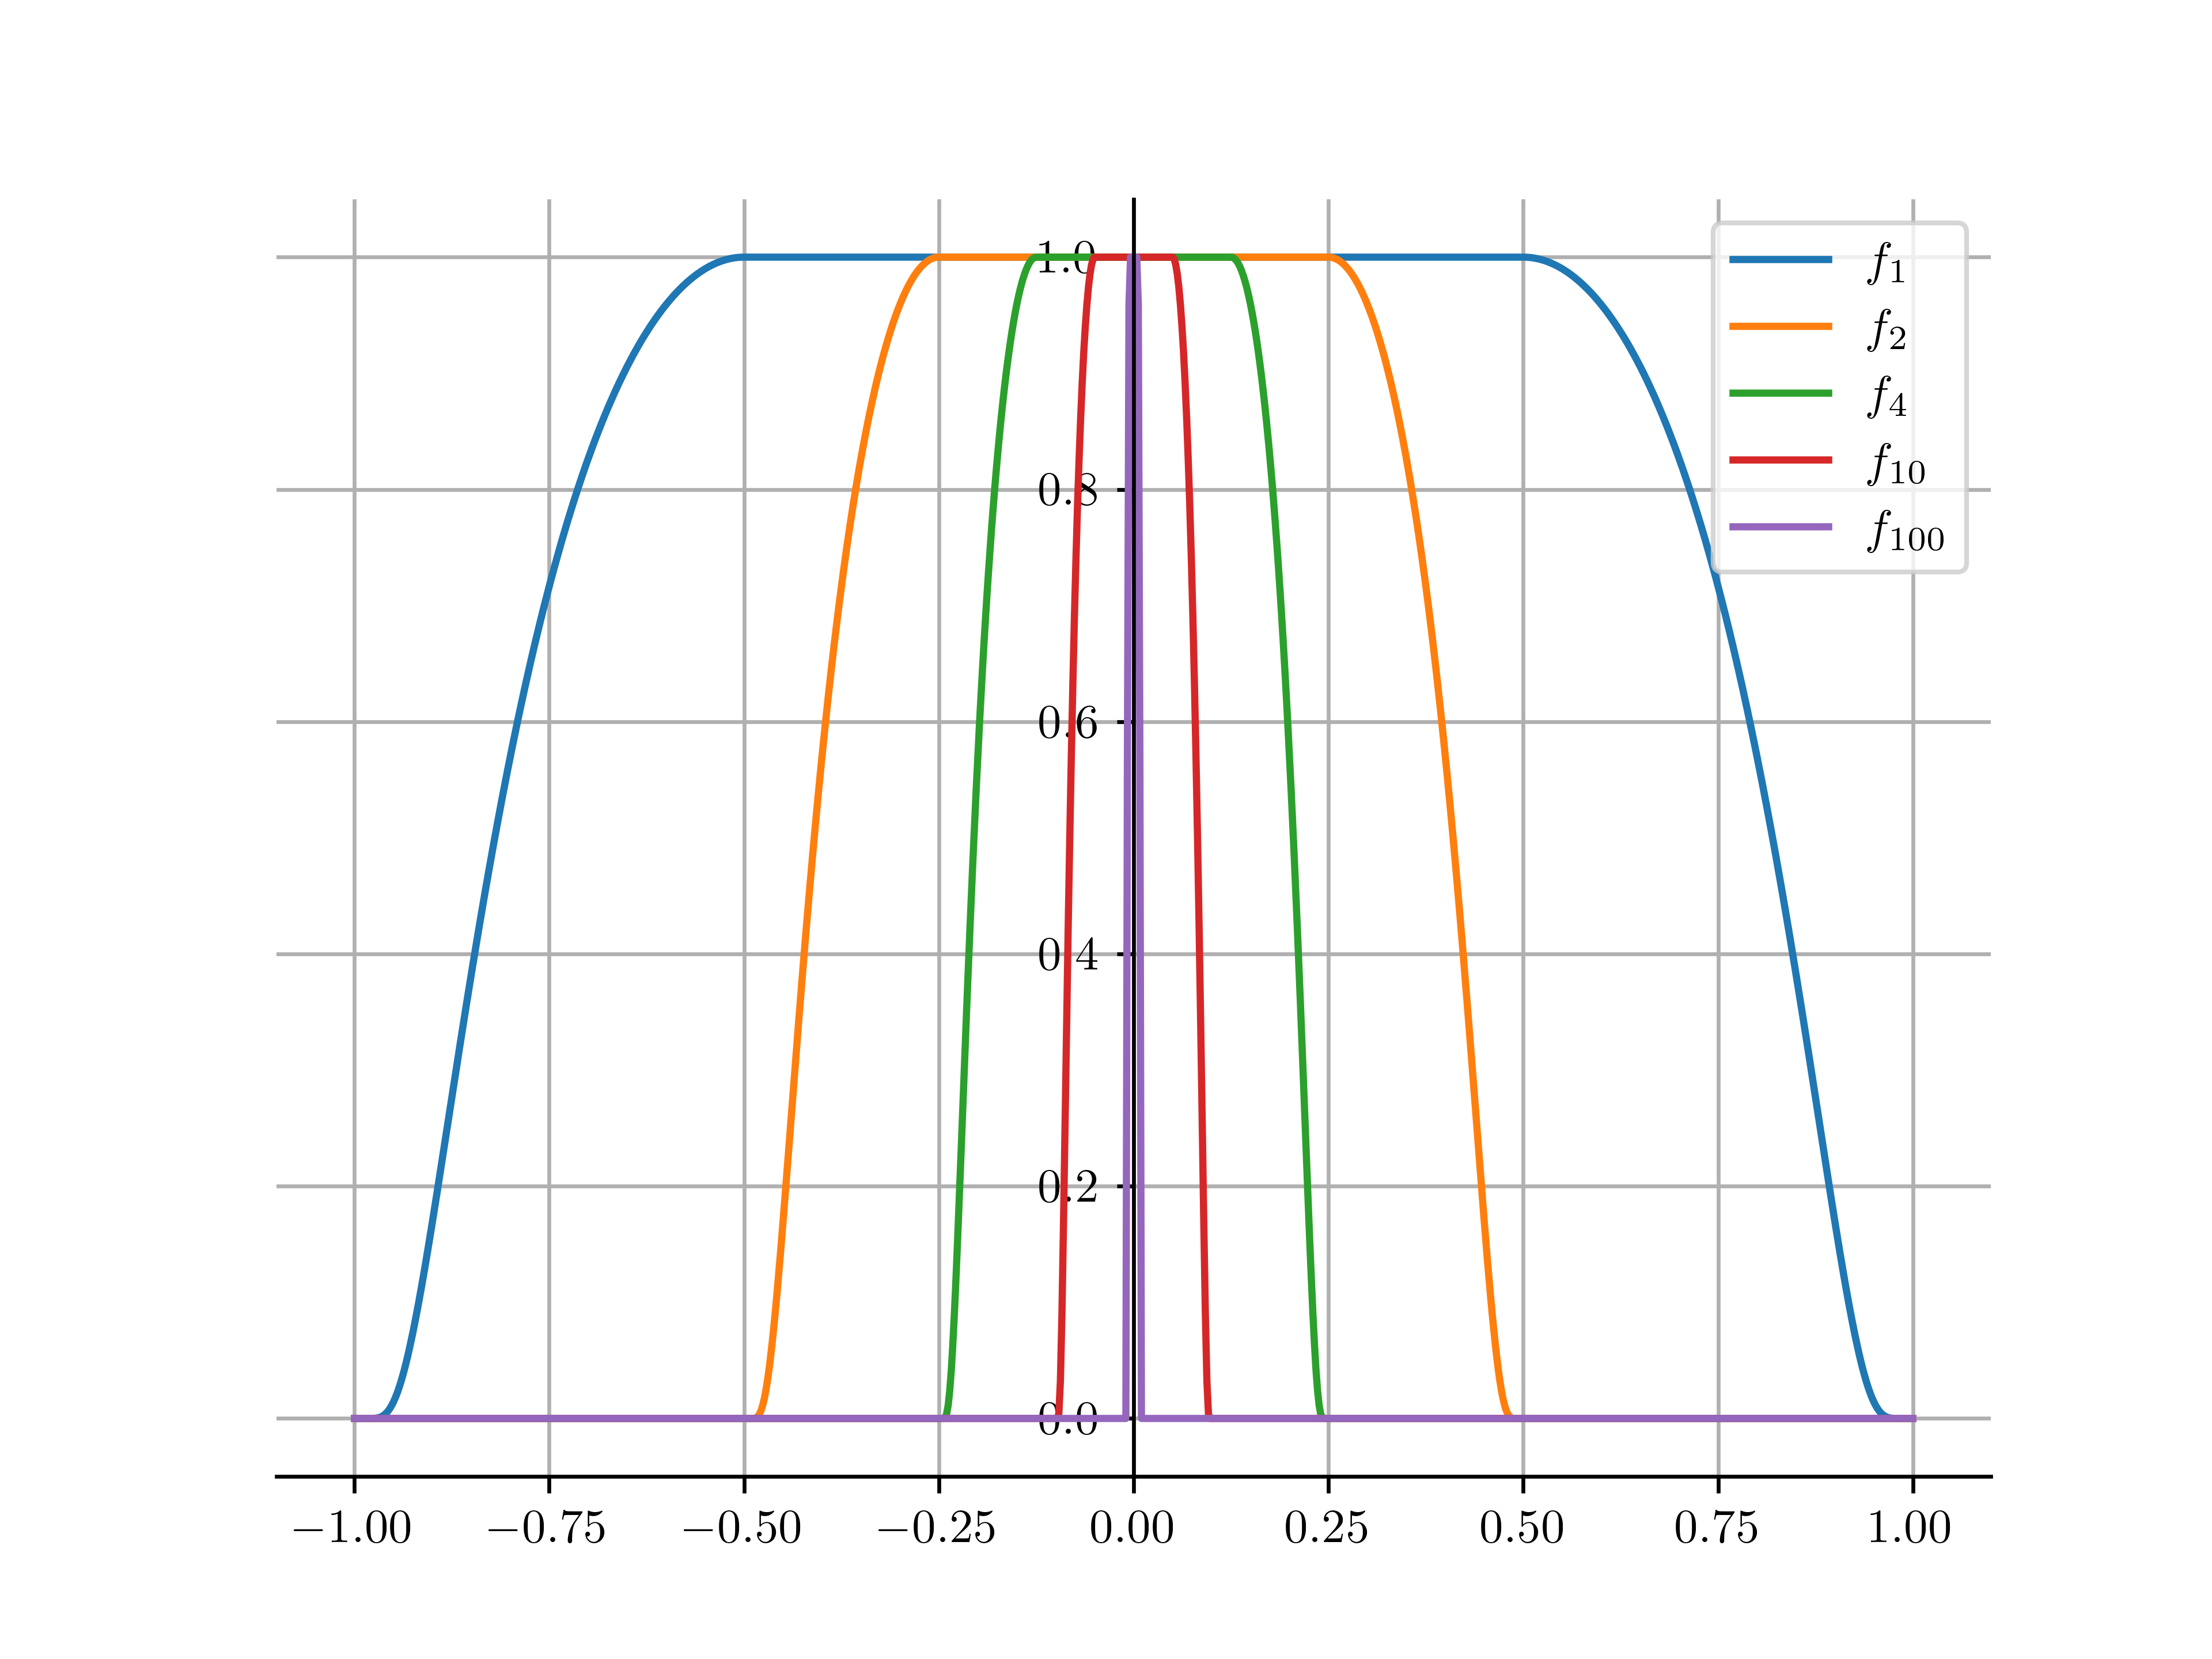
\includegraphics[ width=0.5\paperwidth]{Chapter/Figures/bump_01.png}
  }
  \caption{Example of bump functions}
\end{figure} 



\end{unexaminable}

Recall that we showed unit balls in $\infty$-dimensions are never (sequentially) compact. Weak convergence allows us to restore a weak version of this . %(cf. \todo{})?
For reflexive spaces that is the whole story.  Since $X$ may not be reflexive, one must consider an even weaker topology.  

In the following, we let $(X, \norm{\cdot})$ be a normed linear space, $X^*$ its dual space, $X^{**}$ its bidual, and the isometry $\iota: X \to X^{**}$.  

\begin{definition}
    A sequence of linear functionals $(\ell_n) \subset X^*$ is \textbf{weak*-convergent} to $\ell \in X^*$ if  
    $$
    \lim_{n\to \infty} \ell_n(x) = \ell(x) \qquad \forall x\in X
    $$
    (i.e. pointwise convergence in $X$) Notation: $\ell_n \overset{w^*}{\longrightarrow} \ell$
\end{definition}  

\begin{remark}
\begin{enumerate}[1)]
    \item We now have 3 notions of convergence on $X^*$:
    \begin{enumerate}[i)]
        \item norm/strong convergence: $\norm{\ell_n-\ell}_* \overset{n\to \infty}{\longrightarrow} 0$ (i.e. $\ell_n \to \ell$)
        \item weak convergence: $\ell_n \overset{w}{\longrightarrow} \ell$, i.e.  
        \begin{equation*}
        \forall \xi \in X^{**}: \qquad \lim_{n\to \infty} \xi(\ell_n) = \xi(\ell)    \tag{**}
        \end{equation*}
        \item weak*-convergence: $\ell_n \overset{w^*}{\longrightarrow} \ell$: equivalent to asking $(**)$ for $\xi \in \iota(X)$ only. 
    \end{enumerate}
    \item If $X$ is reflexive $ii) \iff iii)$ [e.g. Hilbert space]
    \item In general, $i) \implies ii) \implies iii)$
\end{enumerate}
    
\end{remark}

\begin{theorem}[Banach-Alaoglu]\nl
\label{Banach-Alaoglu}
Let $X$ be separable. If $(\ell_n) \subset X^*$ is bounded (in $X^*$) there exists $\ell\in X^*$ and a subsequence $\Lambda \subset \natu$ s.t.  
$$
\ell_n \overset{w^*}{\longrightarrow} \ell \qquad n \to \infty, n\in \Lambda
$$
\end{theorem}

\begin{proof}
    Let $(x_j) \subset X$ be a countable, dense subset. Using boundedness, pick a subsequence $\natu \supset \Lambda_1 \supset \Lambda_2 \supset \cdots \supset \Lambda_j \supset \Lambda_{j+1}$ (inductively) such that, for all $j \in \natu$:  
    $$
    \ell_n (x_j) \to a_j \in \real \qquad (n \to \infty, n\in \Lambda_j)
    $$  
    $\Lambda \defeq$ diagonal sequence of $(\Lambda_j)_j$, so $\forall j, \ell_n(x_j) \to a_j, (n\to \infty, n\in \Lambda)$. 
    
    Define $\ell(x_j) \defeq a_j$, extend it linearly on $M = span \{x_j: j\in \natu\}$ and for all $x\in M$:  
    $$
    |\ell(x)| = \lim_{k\to \infty, k\in \Lambda} |\ell_k(x)| \leq \sup_k \norm{\ell_k}_* \norm{x}_{X}
    $$
    so $\ell \in M^*$, hence it can be extended to $\ell \in X^*$ by \Cref{same norm extension}.  

    We now show: $\ell_n \overset{w^*}{\rightarrow} \ell$ $(n \to \infty, n \in \Lambda)$. 
    
    Let $x\in X$, pick $J \subset \natu$ s.t. $x_j \to x$ $(j\to \infty, j \in J)$. For such $j$ and $n\geq 1$:  
    \begin{align*}
        |\ell_n(x)-\ell(x)| &\leq |\ell_n(x-x_j)| + |\ell(x-x_j)| + |\ell_n(x_j)-\ell(x_j)| \\
        &\leq (\sup_n \norm{\ell_n}_* + \norm{\ell}_*) \norm{x-x_j}_X + |\ell_n(x_j)-\ell(x_j)|
    \end{align*}
    Letting first $n\to \infty$ yields  
    $$
    \lim_{n\to \infty, n\in \Lambda} |\ell_n(x)-\ell(x)| \leq C \norm{x-x_j}_X, \qquad j \in J
    $$  
    Now letting $j\to \infty, j\in J$ yields the desired result.
\end{proof}  

\begin{remark}
    \begin{enumerate}[1)]
        \item If $X$ is reflexive, separability can be removed. Together with {\color{red} todo!!!!!!!!!!!}

        \item As a corollary, for $H$ Hilbert. If $(x_n) \subset H$ is bounded ($\sup_n \norm{x_n}_H < \infty$), then $(x_n)$ has a weakly convergent subsequence.  
    \end{enumerate}
\end{remark}

Unless $\dim H<\infty$, one \textbf{cannot} replace weak by strong in 2).

\begin{example}
    \begin{enumerate}[i)]
        \item $X = L^1[0,1]$ is separable, $X^* \cong L^{\infty}$.
        If $(f_n) \subset L^{\infty}$ is bounded, i.e. $\sup \norm{f_n}_\infty < \infty$, \Cref{Banach-Alaoglu} yields a subsequence $(n_k)_k \subset \natu$ and $f\in L^{\infty}$ s.t.  
        $$
        \lim_{k \to \infty} \int f_{n_k}g dx = \int fg dx, \qquad \forall g\in L^1
        $$
        \item $X = L^{\infty}(=L^{\infty}[0,1])$ is not separable (and also not reflexive). The following example shows that the conclusions of \Cref{Banach-Alaoglu} fail in this case. 
        
        For $0<\varepsilon\leq 1$ consider,  
        $$
        T_{\varepsilon}:L^{\infty} \to \real \qquad T_\varepsilon f = \frac{1}{\varepsilon} \int_0^{\varepsilon} f dx, \qquad f\in L^{\infty}
        $$  
        Then $\norm{T_\varepsilon}_{(L^{\infty})^*}\leq 1$, i.e. $T_\varepsilon \in (L^\infty)^*$. We show:  

        \textbf{\underline{Claim:}} $\{T_\varepsilon: 0< \varepsilon \leq 1\}$ is not weak*-sequentially compact.  
        \begin{proof}
            Suppose it is, i.e. $\varepsilon \overset{k  \to \infty}{\longrightarrow} 0$ and $T \in (L^{\infty})^*$ s.t. $T_{\varepsilon_k} \overset{w^*}{\longrightarrow} T$ as $k\to \infty$. By passing to a subsequence, one can assume  
            $$
            1 > \frac{\varepsilon_{k+1}}{\varepsilon_{k}} \to 0 \qquad \text{as\ } k\to \infty
            $$
            Pick $f\defeq \sum_{k=1}^{\infty}(-1)^k \mathbf{1}_{(\varepsilon_{k+1}, \varepsilon_k]} \in L^{\infty}$ with $\norm{f_n}_\infty=1$.  

            For $k\geq 1$, we have:  

            $$
            T_{\varepsilon_k}f = \frac{1}{\varepsilon_k} \sum_{j=k}^{\infty} (-1)^j (\varepsilon_j - \varepsilon_{j+1}) = (-1)^k \frac{\varepsilon_k - \varepsilon_{k+1}}{\varepsilon_{k+1}} +\frac{1}{\varepsilon_k} \int_0^{\varepsilon_{k+1}} f dx
            $$  
            Hence  
            $$
            |T_{\varepsilon_k}f-(-1)^{k}| \leq \frac{1}{\varepsilon_k} \left(\varepsilon_{k+1} + \int_0^{\varepsilon_{k+1}} |f| dx\right) \leq \frac{2\varepsilon_{k+1}}{\varepsilon_k} \overset{k\to \infty}{\longrightarrow} 0
            $$  
            so $(T_{\varepsilon_k} f)_k$ accumulates at $\pm 1$ and is thus divergent.
        \end{proof}

    \item If instead consider $X = C^0[0,1]\subset L^{\infty}$, a separable closed subspace, then \Cref{Banach-Alaoglu} applies to $T_\varepsilon \mid_X$. Indeed, one immediately sees that  
    $$
    T_\varepsilon f \overset{\varepsilon \downarrow 0}{\longrightarrow} f(0), i.e. \qquad T_\varepsilon \overset{w^*}{\rightarrow} \delta_0 \ (\varepsilon \downarrow 0)
    $$
    where $\delta_0$ is the Dirac delta functional at $0$ defined in \Cref{non-reflexive space}.
    \end{enumerate}
\end{example}
\end{document}